\documentclass{article}
% --- Modify margins --- %
\usepackage{geometry}
\geometry{a4paper,scale=0.8}
% --- Involved packages --- %
\usepackage{amssymb}
\usepackage{amsthm}
\usepackage{amsmath}
\usepackage{mathrsfs}
\usepackage{bbm}
\usepackage{graphicx}
\usepackage{listings}
\usepackage{enumitem}
\numberwithin{equation}{section}
\renewcommand\thesection{\Alph{section}}
\counterwithin{figure}{section}
\renewcommand{\thefigure}{\arabic{section}.\arabic{figure}}

% --- Title information --- %
\title{Math 714 - Fall 2020\\
        {\Large \textbf{Homework 1}}
    }
\date{}


% --- main --- %

\begin{document}
    \maketitle
    \section{}
    \begin{enumerate}[label=(\alph*)]
        \item A completely formal computation can be performed for showing this identity, however, first it will be rewritten in a equivalent expression:
        \begin{align*}
            \mu\left(1+\frac{1}{4}\delta^2\right)^{-1/2} &= 1\\
            \mu^2\left(1+\frac{1}{4}\delta^2\right)^{-1}&=1\\
            \mu^2 &= \left(1+\frac{1}{4}\delta^2\right)
        \end{align*}
        Then it is only necessary to show the last equality, in order to do this, the definition of the operator acting on a generic function $u$ will can be used.\\
        Then:
        \begin{align*}
            \mu^2 u(x)
                & = \mu\left(\frac{u(x+h/2)+u(x-h/2)}{2}\right)\\
                & = \frac{u(x+h)+2u(x)+u(x-h)}{4}\\
                & = u(x) + \frac{\delta}{4}(u(x+h/2)-u(x-h/2))\\
                & = u(x) + \frac{\delta^2}{4}u(x)\\
                & = \left(1-\frac{1}{4}\delta^2\right)u(x)
        \end{align*}
        Which shows that the equality holds.

        \item Because we are evaluating the function $u$ in points that are not in the grid.
        \item The typical Taylor expansion were performed
            $$\frac{1}{\sqrt{1+\frac{\delta^2}{4}}} = 1-\frac{1}{8}\delta^2 + \frac{3}{2^7}\delta^2 + \mathcal{O}(\delta^6)$$
        Then, following the instruction we have that
            $$hD = \mu\left(\delta - \frac{1}{6}\delta^3 + \mathcal{O}(\delta^5)\right)$$
    \end{enumerate}


    \section{}
    \begin{enumerate}[label=(\alph*)]
        \item It is clear that for $n = 0$, $D_c$ won’t be consistent in the maximum norm.In fact we have that it diverges, $D_c$ is trying to approximate (in some sense) the derivative of the Heaviside function that is the Dirac delta (in the sense of distributions).\\
        In fact we have that for all $m\not=0$
        \begin{equation}
            D_c x_{+}^0 (-\epsilon) = \frac{(-\epsilon+h)_{+}^0 - (-\epsilon - h)_{+}^0}{2h} = \frac{1-0}{2h}
        \end{equation}
        However,
        \begin{equation}
            D_c x_{+}^0 (-\epsilon) -\frac{d}{dx} x_{+}^0 (-\epsilon) = \frac{1}{2h} - 0 = \frac{1}{2h}
        \end{equation}

        i.e. the error diverges as $h \to 0$, then it is not consistent.

        For $n = 1$ the same computation can be performed, showing that the derivative approximation is exact for all $m \in \mathbb{Z}-\{0,1\}$. In fact for $m = 0,1$ a straight computation shows that:
            $$D_c x_{+}^1 (-\epsilon) = \frac{(-\epsilon+h)_{+}^1 - (-\epsilon - h)_{+}^1}{2h} = \frac{-\epsilon+h-0}{2h}$$
            $$D_c x_{+}^1 (-\epsilon+h) = \frac{(-\epsilon+2h)_{+}^1 - (-\epsilon)_{+}^1}{2h} = \frac{-\epsilon+2h-0}{2h}$$
        If $D_c$ is consistent then as long as $h\to 0$
            $$\frac{-\epsilon+h}{2h} \to 0$$
            $$\frac{-\epsilon + 2h}{2h} \to 1$$

        This means that to have consistence we would need that $\epsilon = h - \mathcal{O}(h^{\alpha})$ with $\alpha > 1$ for the first condition, and $\epsilon = \mathcal{O}(h^{\beta})$ with $\beta>1$ for the second. This is clearly a contradiction, then this scheme can not be consistent for $n=1$.

        For $n \geqslant 2$, is clear that for $m < 0$ the approximation will be exact then the order is infinity, and for $m \geqslant 2$ $D_c x_{+}^n$ is just derivating a polynomial i.e.
        \begin{align*}
            D_c x_{+}^1 (-\epsilon + mh)
            & = \frac{(-\epsilon + mh + h)_+^n - (-\epsilon + mh -h)_{+}^1}{2h}\\
            & = \frac{((-\epsilon+mh)+h)^n - ((-\epsilon+mh)-h)^n}{2h}\\
            & = \frac{(-\epsilon+mh)^n+n(-\epsilon+mh)^{n-1}h - (-\epsilon+mh)^n - n(-\epsilon+mh)^{n-1}h + \mathcal{O}(h^n)}{2h}\\
            & = \frac{2n(-\epsilon+mh)^{n-1}h + \mathcal{O}(h^n)}{2h}\\
            & = n(-\epsilon+mh)^{n-1}+\mathcal{O}(h^{n-1})\\
            & = \frac{d}{dx}(-\epsilon+mh)_{+}^n + \mathcal{O}(h^{n-1})
        \end{align*}
        Then for $m\geqslant 2$ the approximation is of order $n-1$.

        The special cases are studied separately
        \begin{align*}
            D_c x_{+}^1 (-\epsilon)
            & = \frac{(-\epsilon + h)_{+}^n - (-\epsilon - h)_{+}^1}{2h}\\
            & = \frac{(-\epsilon + h)^n}{2h}\\
            & = 0 + \mathcal{O}(h^{n-1})\\
            & = \frac{d}{dx}(-\epsilon)_{+}^n + \mathcal{O}(h^{n-1})
        \end{align*}
        because by definition $0<\epsilon<h$
        \begin{align*}
            D_c x_{+}^1(-\epsilon + h)
            & = \frac{(-\epsilon + 2h)_{+}^n - (-\epsilon)_{+}^1}{2h}\\
            & = \frac{(-\epsilon + 2h)^n}{2h}\\
            & = n(-\epsilon+h)^{n-1} + \mathcal{O}(h^{n-1})\\
            & = \frac{d}{dx}(-\epsilon+h)_{+}^n + \mathcal{O}(h^{n-1})
        \end{align*}
        Then the scheme is accurate of order $n-1$ in $l^\infty$-norm.
        \item If $m$ is finite, by equivalence of norms ts is known that
        \begin{equation}
            h||u||_\infty \leqslant ||u||_1 \leqslant Ch||u||_\infty
        \end{equation}
        Then if the scheme was $n$-th order accurate with the $l^\infty$-norm, then it will be $n+1$-th order accurate with the $l^1$-norm. i.e. for $n \geqslant 2$ the scheme will be consistent and of $n$-th order accurate with the $l^1$-norm.

        For the special case, $n = 0$ the $l^\infty$-norm is $\frac{1}{2}h$, then the $l^1$-norm of the error si bounded by below by $\frac{1}{2}$, then the scheme is not consistent.

        For $n = 1$,  the $l^\infty$-norm is dominated by:
            $$\left\Vert D_c - \frac{d}{dx}x_{+}^n \right\Vert_{l^\infty} = \max{\left(\frac{-\epsilon+h}{2h}, \frac{-\epsilon+2h}{2h}\right)}$$
        then using the right part of eq. B.3
            $$\left\Vert D_c - \frac{d}{dx}x_{+}^n \right\Vert_{l^1} = C\max{\left(\frac{-\epsilon+h}{2}, \frac{-\epsilon+2h}{2}\right)}\to 0$$
        Then for $n=1$ the scheme is consistent and first order accurate.

        \item The normal Taylor expansion argument, gives an upper bound given by the $h^2$ times the $L^\infty$-norm, over a compact set of the third derivative of $u$.
        
        In this case we have that for $n=3$,
            $$\frac{d}{dx^3}x_{+}^3 = 6H(x)$$
        where $H(x)$ represents the Heaviside function, in fact this function is not continuous, however the statement is still true. Because we can still use the Integral remainder for finite Taylor expansions. And for this it is only needed that the third derivative is integrable, and in this case it is.

        Then a Taylor expansion argument using the Integral remainder gives us that
        
        $$\left\Vert D_c x_{+}^3 - (x_{+}^3)' \right\Vert_{l^\infty} = \mathcal{O}(h^2)$$

        And in the last question it was proven that for $n =3$ the operator $D_c$ was second order accurate, then this arguments gives us just the right order of accuracy.
    \end{enumerate}


    \section{}
    \begin{enumerate}[label=(\alph*)]
        \item The simplest way to discretize the laplacian is a five point stencil scheme, in fact the approximation of the second derivative are made by a centered three point stencil in each direction, in other words:
        \begin{align*}
            \frac{\partial^2 u(x_{i,j})}{\partial x^2}
            & \approx \frac{u(x_{i+1,j})-2u(x_{i,j})+u(x_{i-1,j})}{h_{x}^2}\\
            \frac{\partial^2 u(x_{i,j})}{\partial x^2}
            & \approx \frac{u(x_{i,j+1})-2u(x_{i,j})+u(x_{,j-1})}{h_y^2}
        \end{align*}
        where $h_x$ and $h_y$ are the space stepping in each direction, and $n$ and $m$ are the number of unknowns in each direction respectively, then the discretized laplacian is given by
            $$-\Delta u(x_{i,j}) = \frac{4u(x_{i,j})}{h_x^2+h_y^2} - \frac{u(x_{i+1,j})u(x_{i-1,j})}{h_x^2} - \frac{u(x_{i,j+1})+u(x_{i,j-1})}{h_y^2}$$
        From this observation it is easy to see that the laplacian is equivalent in this case a two 1D laplacians in each direction. In fact we have that:
            $$\tilde{\Delta} = A \otimes I + I \otimes B$$
        where $A$ is the typical $n \times n$ matrix given by
        \begin{align*}
            A = \frac{1}{h_x^2}\begin{pmatrix}
                2 & -1 & 0 & \cdots & \cdots & 0\\
                -1 & 2 & -1 & 0 & \cdots & \vdots\\
                0 & \ddots & \ddots & \ddots & \ddots & .\\
                \vdots & \cdots & -1 & 2 & -1 & 0\\
                \vdots & 0 & \cdots & -1 & 2 & -1 \\
                0 & \cdots & \cdots & 0 & -1 & 2
            \end{pmatrix}
        \end{align*}
        And for $B$ is the same matrix than $A$ plus two extra unknowns, that are the ones used to closed the linear system and imposing the condition of zero derivative at the boundary, then $B$ is given by:
        \begin{align*}
            B = \frac{1}{h_y^2}\begin{pmatrix}
                \frac{3}{2}h_y & -2h_y & \frac{1}{2}h_y & 0 & \cdots & 0\\
                -1 & 2 & -1 & 0 & \cdots & \vdots\\
                0 & \ddots & \ddots & \ddots & \ddots & .\\
                \vdots & \cdots & -1 & 2 & -1 & 0\\
                \vdots & 0 & \cdots & -1 & 2 & -1 \\
                0 & \cdots & 0 & \frac{1}{2}h_y & -2h_y & \frac{3}{2}h_y
            \end{pmatrix}
        \end{align*}
        \item In this case a quite simple anzat for the exact solution can be used, taking in account the boundary condition, a solution of the elliptic problem should have the form:
            $$u(x,y) = \cos{(2\pi x)}\alpha(y)$$
        Then,\begin{align*}
            \Delta u(x,y) 
            & = -(2\pi)^2\cos{(2\pi y)}\alpha(x) + \cos{(2\pi y)}\alpha'' (x)\\
            & = \cos{(2\pi y)}(\alpha'' (x) - (2\pi)^2\alpha(x))\\
            & = 0
        \end{align*}
        i.e.
        \begin{align*}
            \alpha'' (x) - (2\pi)^2\alpha(x) &= 0\\
            \alpha(0) & = 1\\
            \alpha(1) & = 0
        \end{align*}
        the answer for this ODE is
            $$u(x,y) = \cos{(2\pi y)}\left[-\frac{1}{e^{4\pi}-1}e^{2\pi x} + \frac{e^{4\pi}}{e^{4\pi -1}}e^{-2\pi x}\right]$$
        To compute the Numerical Approximation a Gauss-Siedel iteration as used, at each iteration the boundary conditions are imposed. Then the next approximation is computed inside the domain, here we show the main MATLAB loop.
        \lstinputlisting[language=MATLAB]{C2.m}
        The numerical solution is compared against the analytic solution, this error is produced by the contribution of two different kind of errors. The first one, is the error coming from the discretization of the PDE, and it is second order in $h$ if the solution is enough smooth. The second one, is the error arising from the fact that the solution to the linear system is computed using an iterative solver. In fact this can be seen, in fig. 3.1. At the beginning the error is from the iterative solver, and this decreases until it stabilizes. And this error is the error given by the FD scheme.
        \begin{figure}[!htbp]
            \centering
            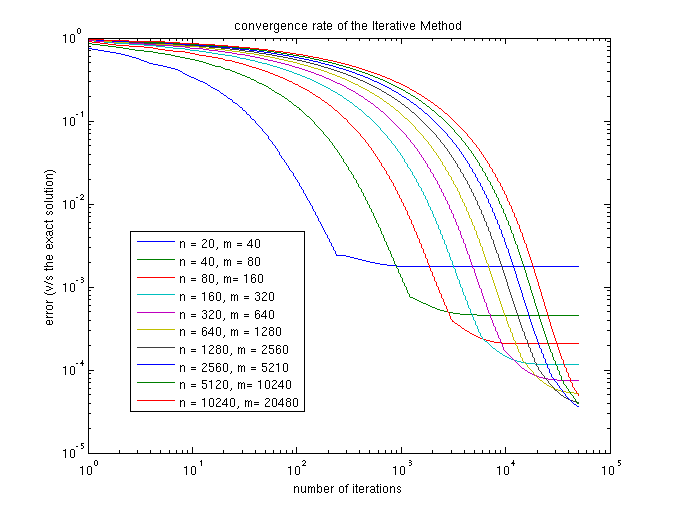
\includegraphics[width=15cm]{./p-set1/inform-1.png}
            \caption{Error ($v/s$ exact solution) of the GS iteration}
        \end{figure}
        To prove that the scheme is consistent, the error of the iterative method must be significantly smaller. For this the solver is iterated until getting convergence.

        It is possible to see in the fig. 3.1 that the bigger the system is, slower the information is transmitted from the boundary to the interior of the domain, and then slower the convergence rate becomes. In fact increasing the number of unknowns does not give a significant gain, because the convergence rate become significantly small.

        \begin{figure}[!htbp]
            \centering
            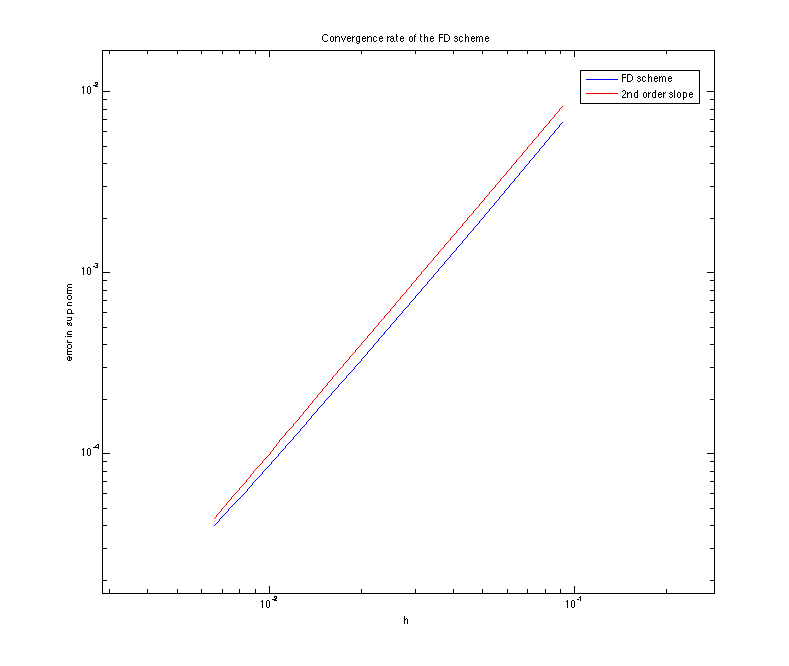
\includegraphics[width=15cm]{./p-set1/inform-2.png}
            \caption{Error $v/s$ space step $h_x = \frac{1}{2}h_y$}
        \end{figure}

        For getting the fig. 3.2, all the points shown are the result after the stabilization of the error. It is possible to see that the scheme is in fact of second order (red line) as expected.
        \item In fact, the error goes to zero as expected, then the scheme is consistent. The solution $u$ is $\mathcal{C}^{\infty}$ because, the domain is a bounded convex polygon, and all the data are smooth, then by elliptic regularity (and Sobolev embeddings) the solution is smooth.
    
        \item The eigenvalues are of the form $\lambda_{-\tilde{\Delta}} = \lambda_A + \lambda_B$ and the eigenvectors will have the form of $v_{-\tilde{\Delta}} = v_A \otimes v_B$ this is just using the properties of the Kronecker product.
        
        In fact:\begin{align*}
            -\tilde{\Delta} \cdot v_{-\tilde{\Delta}}
            & = (A \otimes I + I \otimes B) \cdot (v_A \otimes v_B) \\
            & = A \otimes I \cdot v_A \otimes v_B + I \otimes B \cdot v_A \otimes v_B\\
            & = (A \cdot v_A) \otimes (I \cdot v_B) + (I \cdot v_A) \otimes (B \otimes v_B)\\
            & = (\lambda_A v_A) \otimes (v_B) + (v_A) \otimes (\lambda_B v_B)\\
            & = (\lambda_A + \lambda_B)(v_A \otimes v_B)\\
            & = \lambda_{-\tilde{\Delta}}v_{-\tilde{\Delta}}
        \end{align*}

        \item The minimum eigenvector of $-\tilde{\Delta}$ is given by $\lambda_{\min}(A) + \lambda_{\min}(B)$ , by the last question.
        
        It is know that $\lambda_{\min}(B) = 0$ that is the eigenvalue associated to the constant function, for every $h_y$. However it is know that $\lambda_{\min}(A) = \frac{4}{h_y^2}\sin^2{(\frac{\pi h_y}{2})}$.

        Then using Taylor expansion it can be shown that this quantity is bounded by below for every $h \ll 1$. In fact:
        \begin{align*}
            \frac{4}{h_y^2} \sin^2{(\frac{\pi h_y}{2})}
            & = \frac{4}{h_y^2}\left(\frac{\pi h_y}{2}-3!\left(\frac{\pi h_y}{2}\right)^3 + \mathcal{O}(h^5)\right)^2\\
            & = \frac{4}{h_y^2}\left(\left(\frac{\pi h_y}{2}\right)^2 - 3!\left(\frac{\pi h_y}{2}\right)^4 + \mathcal{O}(h^6)\right)\\
            & \geqslant \frac{1}{2}\frac{4}{h_y^2}\left(\frac{\pi h_y}{2}\right)^2\\
            & = \frac{1}{2}\pi^2
        \end{align*}
        Then $C = \frac{1}{2}\pi^2$.
        \item The criteria for convergece was the stabilization of the numerical soltuion between two loops, in others words;
            $$\left\lVert u^{k+1} - u^k\right\rVert_{l^\infty} < 10^{-10}$$
        Using this the follow graph is obtained
        \begin{figure}[!htbp]
            \centering
            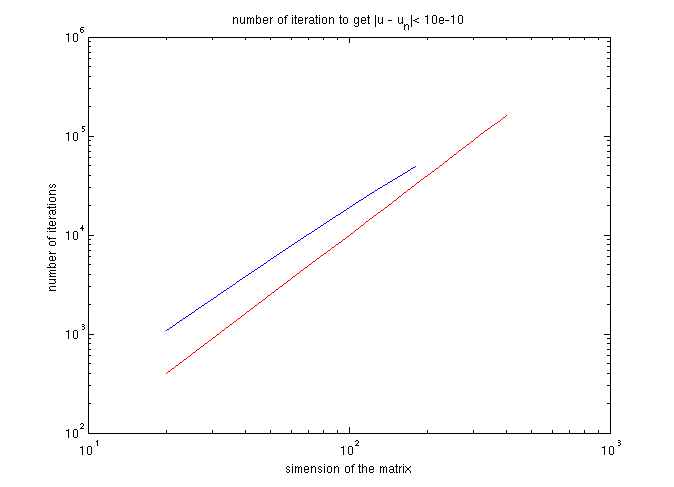
\includegraphics[width=15cm]{./p-set1/inform-3.png}
            \caption{Number of iteration until getting convergence of the approximated solution (blue) and theoretical estimation (red)}
        \end{figure}

        it is possible to appreciate that the slope of the numerical approximation is in some sense near the theoretical asymptotic result, that is $\mathcal{O}(n^2)$
        \item The order of convergence becomes sub linear, because in this case a Taylor expansion is not permitted because the boundary data is not $\mathcal{C}^{\infty}$, then the solution
        will be smooth in the interior of the domain, because  $0 = f \in \mathcal{C}^{\infty}$, however in the boundary it will be in $L^2(\partial\Omega)$ and in dimension 1 this space is not embedded in $\mathcal{C}^0$.

        Then, the argument given by the Taylor expansion is not valid anymore.

        \begin{figure}[!htbp]
            \centering
            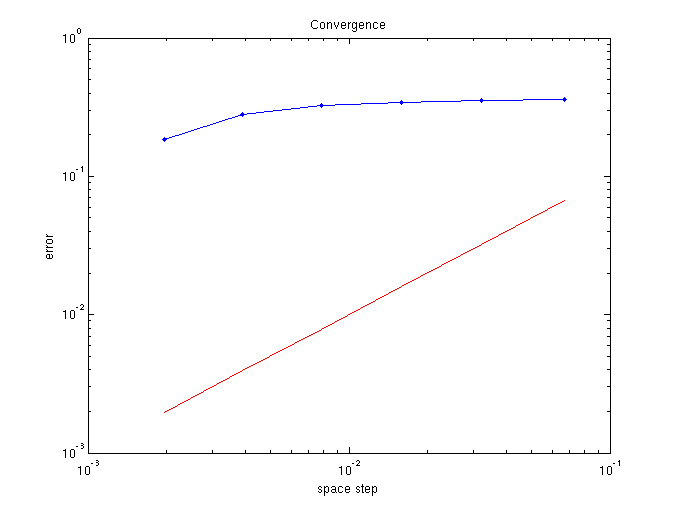
\includegraphics[width=15cm]{./p-set1/inform-4.png}
            \caption{Error $v/s$ space step $h_x = h_y$ for discontinuous boundary condition}
        \end{figure}

        The fig. 3.4 was made using as a reference a solution for a grid of dimention $n = m = 1024$. It is clear that the method converges in an sublinear order in the $l^{\infty}$ norm, however it converges linearly in $l^2$, fact that is not showed here.
    \end{enumerate}


    \section{}
    A Multigrid method, using V-cycles, for solving the linear system was implemented, for illustrate the gain in convergence speed the standard procedure is by count of the number of operations. However, this approach represents some complication, because of the nested loops, then a time-benchmark strategy was implemented.
    The results are shown in fig.4.1.

    \begin{figure}[!htbp]
        \centering
        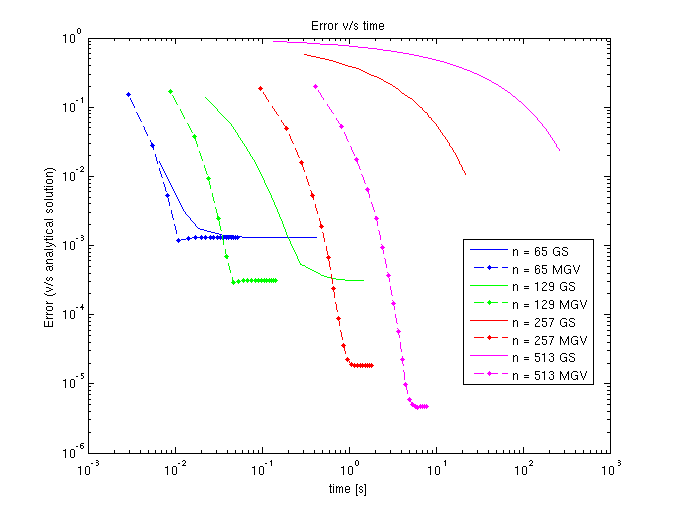
\includegraphics[width=15cm]{./p-set1/inform-5.png}
        \caption{Speed gain, between Gauss-Siedel and Mulgrid V-cycles}
    \end{figure}

    As expected, as $n$, the size of the dimesion of the grid, increases, the gain becomes more evident.


\end{document}